% ****************************************************************
\newpage
\section{Gradient Descent}
\label{sec:gradient_descent}

\begin{flushleft}

Gradient Descent ist ein Optimierungsalgorithmus, um ein lokales Minimum einer Funktion zu finden.
Gegeben sei eine Kosten-Funktion $J(\Theta_{0}, \Theta_{1})$, gesucht ist das Minimum der Funktion $min_{\Theta_{0}, \Theta_{1}} J(\Theta_{0}, \Theta_{1})$, indem die Parameter $\Theta_{0}$ und $\Theta_{0}$ laufend ein wenig verändert werden.

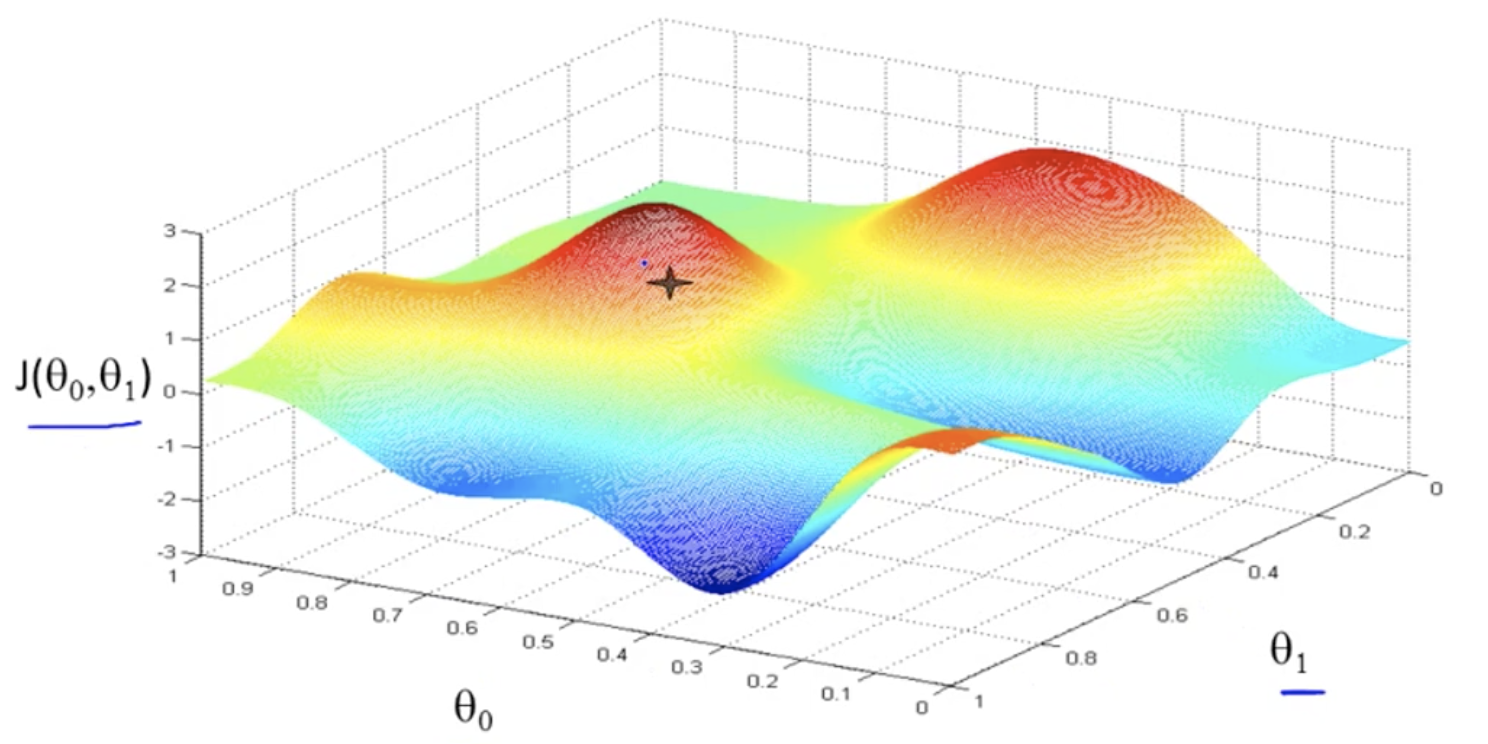
\includegraphics[scale=0.6]{figures/gradient_descent}

Wiederholen bis zur Konvergenz:
$$\Theta_{i} := \Theta_{i} - \alpha\frac{\partial}{\partial \Theta_{i}} J(\Theta_{0}, \Theta_{1}) $$

$$ \alpha: Learning Rate $$
$$ i=0, i=1 $$

\subsubsection{GD für Linear Regression}
Model Funktion:
$$h_{\Theta} = \Theta_{0} + \Theta_{1}x$$
Cost-Function:
$$ J(\Theta_{0}, \Theta_{1}) = \frac{1}{2m} \sum_{i=1}^{m}(h_{\Theta}(x^{(i)})-y^{(i)})^{2} $$

Für lineare Regression hat die Kostenfunktion stets nur ein lokales (sprich globales) Minimum.
\linebreak
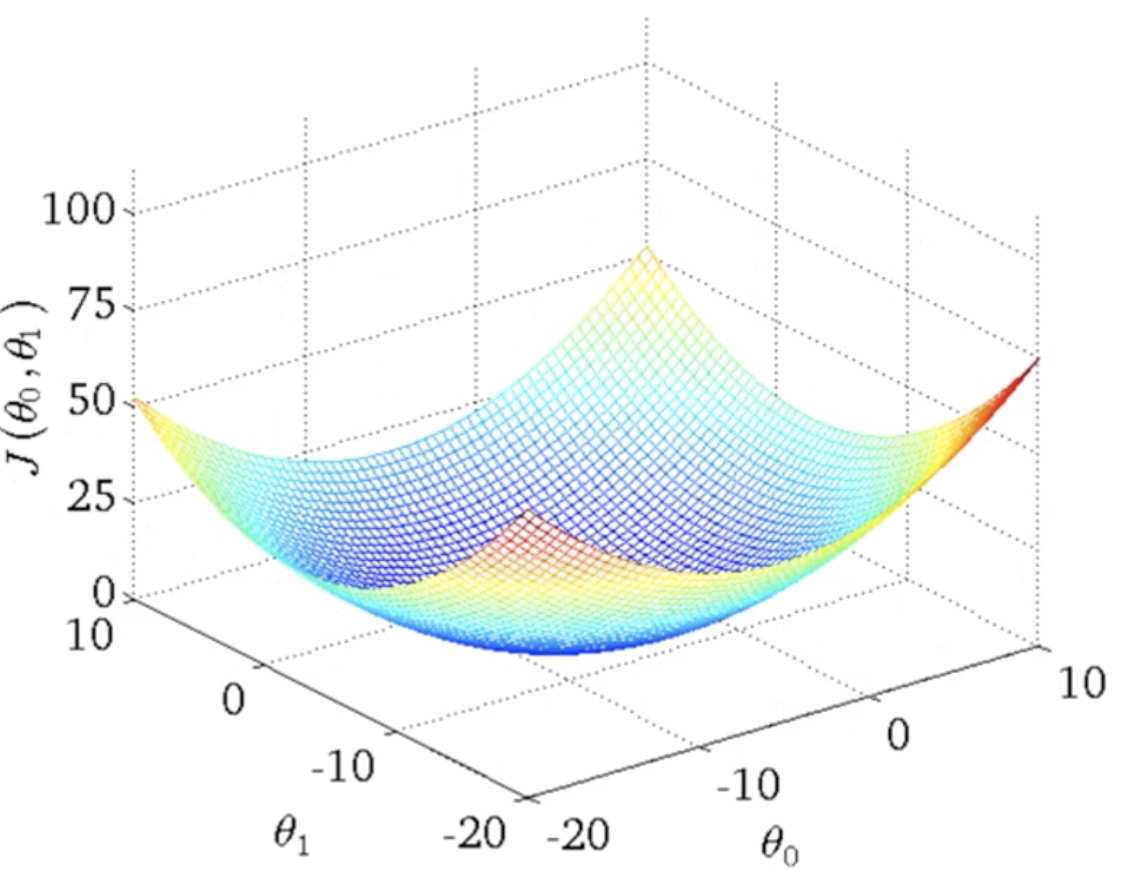
\includegraphics[scale=0.6]{figures/cost_function_linear_regression}
\linebreak
Der Gradient Descent Algorithmus für eine simple Lineare Regression rechnet sich wie folgt:
\linebreak


\begin{algorithm}
\caption{Calculate $\text{min}_{\Theta} J(\Theta)$}
\begin{algorithmic} 
\Repeat 
\State $ \Theta_{0} := \Theta_{0} - \alpha \frac{1}{m} \sum_{i=1}^{m}(h_{\Theta}(x^{(i)}) - y^{(i)}) $

\State $ \Theta_{1} := \Theta_{1} - \alpha \frac{1}{m} \sum_{i=1}^{m}(h_{\Theta}(x^{(i)}) - y^{(i)})*x^{(i)} $
\Comment{simultaneously update all $\Theta_{j}$}
\Until{$J(\Theta_{0}, \Theta_{1})$ converges}
\end{algorithmic}
\end{algorithm}


\end{flushleft}
% ****************************************************************


